\fancychapter{Evaluation Metrics}
\label{ch:eval_met}
On this chapter, we will start by describing the results of \ac{SOM} for clustering topics on twitter. The following section will be dedicated to analyze the work done on \ac{VSM} reduction with tweets.
Section~\ref{sec:som_framework}, will describe particular parts, and benchmark the training process with generic RGB vectors on the \ac{SOM} framework. Finally we will show the results of clustering tweets, with our tweaks applyed to the \ac{SOM} algorithm --- The Homophilic \ac{SOM}.

\section{Clustering Tweets with Self-Organizing Maps}
\label{sec:clustering_tbla}
This section is dedicated to the evaluation of clustering tweets with the default \ac{SOM} algorithm. We also benchmarked the application of string reduction techniques to the \ac{VSM}.  

\subsection{SOM training}
\label{sub:clustering_tweets_with_soms}
Our first approach to cluster tweets with \ac{SOM} started by dynamically creating \ac{VSM} for each new word that was encountered while scanning each tweet on the dataset. Due to simplicity of the approach, an overwhelming amount of different words, some even without any clear meaning, took relevance on the \ac{VSM}. 
This created a \ac{VSM} with a huge size and the trainings at hand took an eternity to process. In order to prevent this from happening, we took a sample of 50MB of tweets, all in English, from the dataset and started to train the \ac{SOM} with it. String manipulation for \ac{VSM} reduction described on Subsection~\ref{sub:clustering_tweets} were used.
The \ac{SOM} training was performed using the R kohonen package~\cite{rsom}. We have added some information about this train on Appendix~\ref{ch:rsom_training}, three kinds of clusters were found: clusters where no topic could be made sense of, clusters with one or more topics and clusters with a ton of tweets which had the same text . An example of tweets present in these clusters can be seen in Figures \ref{fig:cluster1}, \ref{fig:cluster2} and \ref{fig:cluster3}, respectively.  

\begin{figure}[h!]
  \centering
  \subfigure[Cluster without topics]{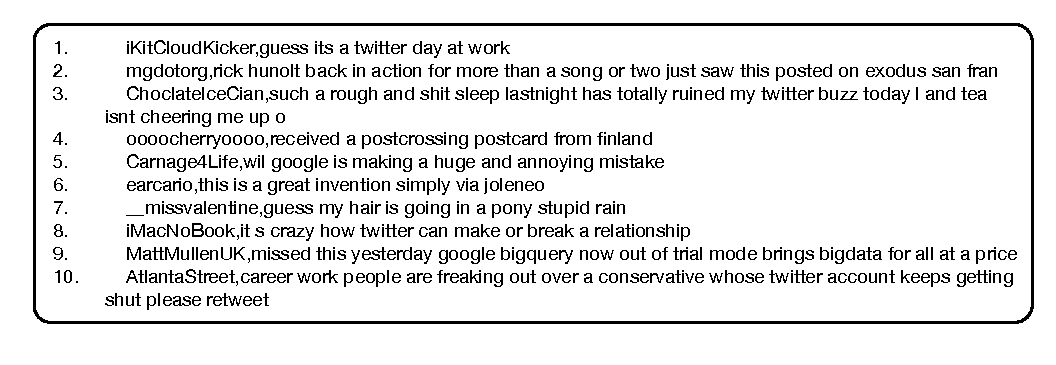
\includegraphics[scale=0.6]{./images/clutercluster.pdf}\label{fig:cluster1}}
  \hspace*{0.5cm}
  \centering
  \subfigure[Cluster with the iPad topic]{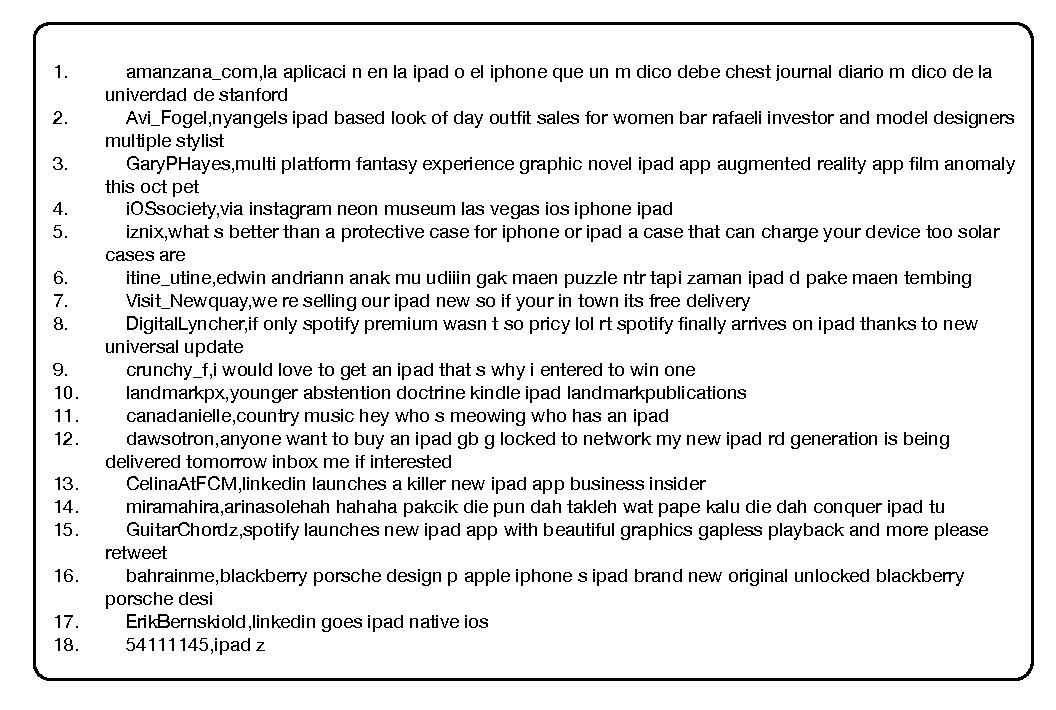
\includegraphics[scale=0.6]{./images/ipadcluster.pdf}\label{fig:cluster2}}
  \hspace*{0.5cm}
  \centering
  \subfigure[Cluster with autumaticlly generated text]{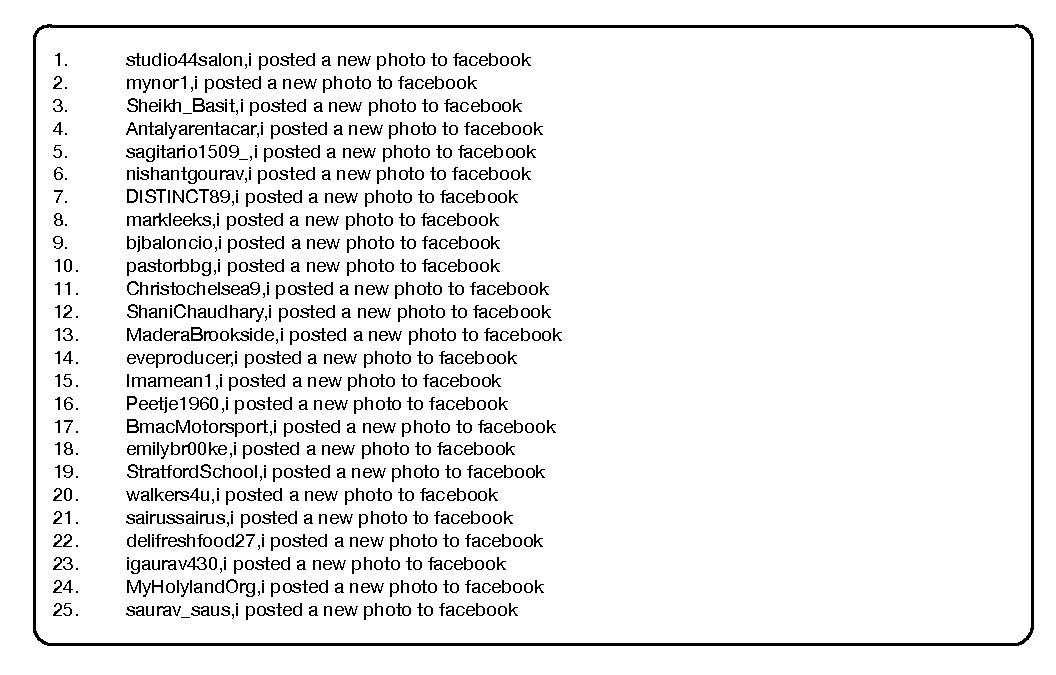
\includegraphics[scale=0.6]{./images/facecluster.pdf}\label{fig:cluster3}}
  \caption{Three types of clusters}
\end{figure}

\subsection{Reducing SOM vector size}
\label{sub:reducing_som_vector_size}
In Subsection~\ref{sub:clustering_tweets}, we introduced string reducer methods which enabled great \ac{VSM} reduction. On Figure~\ref{fig:plot_word_red}, we can see the amount of words removed by each method alone, and by all methods combined --- column "All Methods". In order to build this graph, we applied each method independently to a sample of 902802 tweets.

\begin{figure}[htpb]
  \centering
  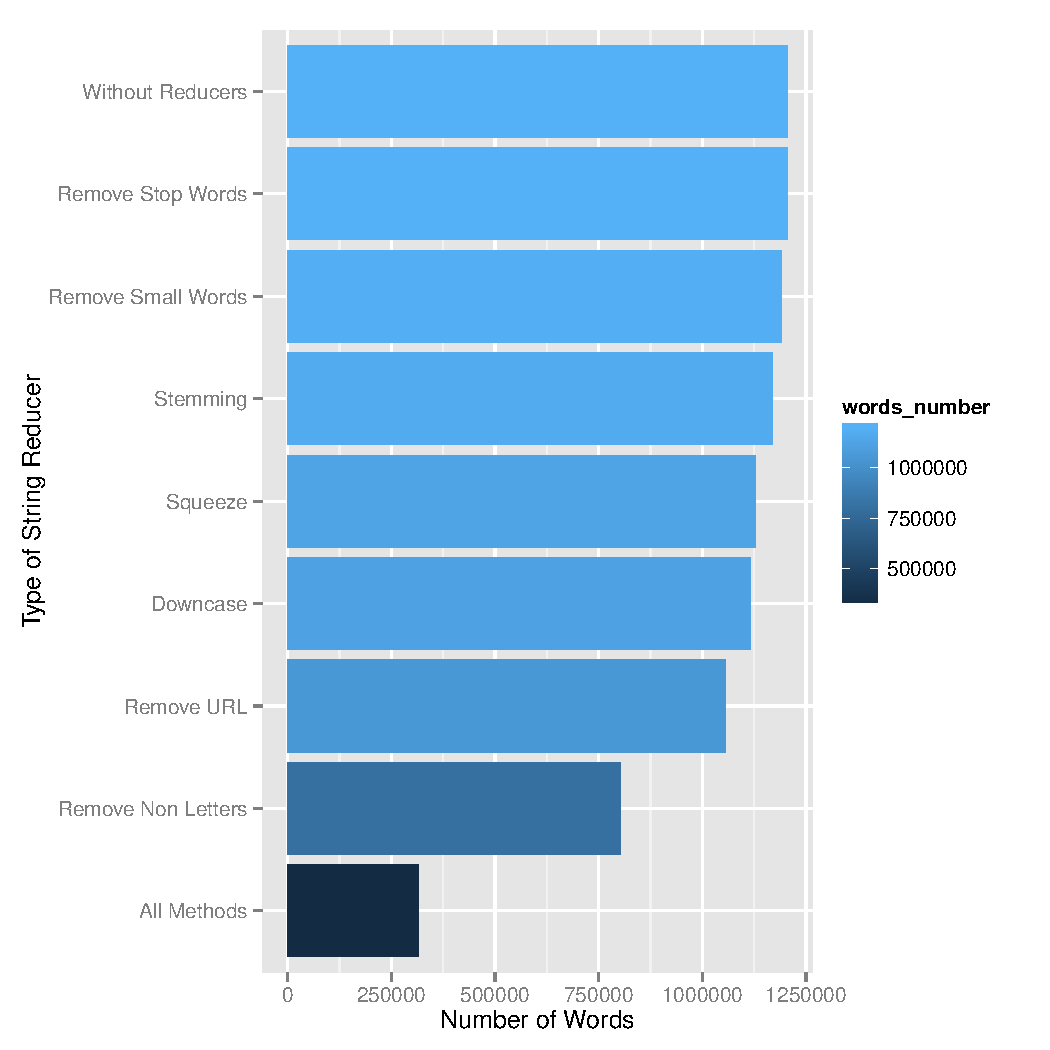
\includegraphics[width=0.8\linewidth]{./plots/svm/plot_wordcount.pdf}
  \caption{Amount of unique words present on dataset sample with 902802 tweets, based on the string word reduction technique applied.}
  \label{fig:plot_word_red}
\end{figure}

It is interesting to see that each method by itself doesn't remove a great amount of words. The method that removed more words by itself was "remove non letters" --- which removes every character that is not a letter ---, at an order of 33\%. On the other hand, the method "remove stop words" by itself removed only 400 of words. This was expected due to the fact that the full list of MySQL stop words used by this method only has 543 words. All methods combined were able to reduce the \ac{VSM} size in about 75\%.

String reduction techniques work directly with text and has no notion whatsoever of linguistic semantics. In Subsection~\ref{sub:tweeter_natural_language_processing}, we presented a twitter \ac{NLP} library which can be used effectively to understand the linguistic semantics used on twitter. 

By feeding the same dataset as used above to the library, we were able to identify multiple types of words that can afterwards be considered relevant for~\ac{TDT}. On Figure~\ref{fig:wordcount_nlp}, the red bars show the amount of unique words found under a specific semantic tag, whilst in blue we can see words tagged under the same category after applying string reduction techniques.

Due to the fact that we are trying to identify topics, most of the tagged words are of no use. We chose to use only common nouns, proper nouns and hashtags during the clustering process. By applying all these filters to the dataset sample, we have a \ac{VSM} reduction of about 90\%, from 1 204 743 different words to 132 861.

\begin{figure}[htpb]
  \centering
  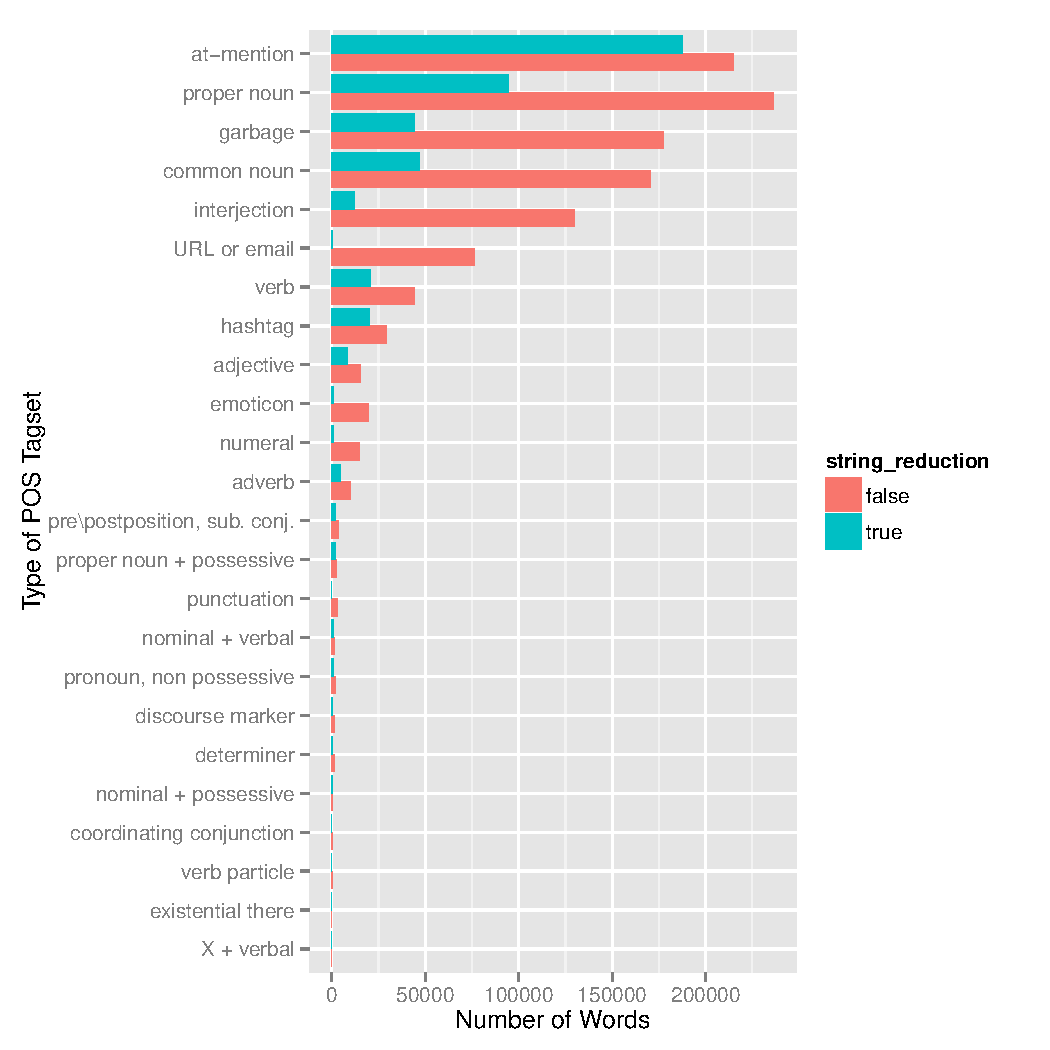
\includegraphics[width=0.8\linewidth]{./plots/svm/plot_wordcount_nlp.pdf}
  \caption{Number of words tagged with Ark Tweet NLP. In red we can see the number of unique words tagged in each category, while in blue we can see the amount of unique words, after applying string reduction techniques.}
  \label{fig:wordcount_nlp}
\end{figure}

\subsubsection{Identify Tweets language}
\label{ssub:identify_tweets_lang}
Twitter is a social network with users from every corner of the world, thus tweets tend to be in a lot of different languages. Twitter internationalization greatly affects the clustering process, with multi language synonyms and idiomatic expressions. Another problem is associated with results interpretation, when a cluster is formed with tweets with languages foreign to the people who are analyzing the results. When this happens, identifying topics on the cluster is extremely hard, and most of the times the researcher will have to manually translate a cluster.  

One way to infer a tweet language, is by looking at the language which a user has on his twitter profile, through the twitter API. Some times, users use their profiles on different languages than the language in which they issue their tweets, which makes the process of excluding foreign tweets harder.

An alternative approach to language identification, is by using an external library like whatlanguage~\footnote{https://github.com/peterc/whatlanguage}, which tries to identify one language through the usage of Bloom Filters.  

In order to better understand the relationship between a tweet language and a user profile language, we analyzed a sample of 87 tweets, all from different users and categorized their language by hand. We found that 7 users were using an English profile, and tweeting in other language.

On the same sample, we used the language identification library and found that even though only 8 tweets were identified as being in English, it did not misidentified any foreign tweet as being in English. The results of the queries conducted in the sample can be found on Table~\ref{tab:mac_test}.  

\begin{table}[H]
  \caption{Tweets language detection summary }
  \label{tab:mac_test}
  \begin{center}
    \begin{tabular}{|c|c|}
      \hline
      Total amount of tweets gathered      & 87  \\
      \hline
      \hline
      Tweets with user language and tweet language in english      & 25  \\
      \hline
      Tweets with user language and tweet language not in english      & 7  \\
      \hline
      \hline
      Tweets tagged in english and tweet language was in english      & 8  \\
      \hline
      Tweets tagged in english and tweet language was not       & 0  \\
      \hline
    \end{tabular}
  \end{center}
\end{table}


Even though the sample is quite small, it was possible to understand that selecting only tweets with English profiles and afterwards selecting only the ones identified in English by the language identification library, could yield a bigger number of false negatives --- tweets in English which were thought to be in other language ---  , but would help prevent selecting tweets that were not in English.

\subsection{Conclusions}
\label{sub:conclusions}
Reducing the \ac{VSM} size by string reduction and tweet language identification greatly improved the results of topic detection on the dataset at hand. Mainly by removing characters without meaning, and by making similar words equal. The next step in detecting topics on twitter will be to modify the \ac{SOM} algorithm, but first we need to build a twitter crawler. 

\section{Twitter Crawler}
\label{sec:twitter_crawler}
After analyzing the work accomplished by clustering tweets on Section~\ref{sec:clustering_tbla}, we decided that some alterations to the algorithm should be done in order for it to take into account the social connections between the data. In order to accomplish this we needed a dataset with social connections behind the authors of the tweets. There was two ways to accomplish this: 

\begin{itemize}
  \item \textbf{First aproach: } For each tweet we have on our dataset, fetch the user information including the users he is connected to.
  \item \textbf{Second aproach: } Create our own crawler, where the social connections, tweets and users are saved.
\end{itemize}                                                                                             
We followed the second approach in order to have more control over the data used from this moment forth, and to have a better integration of the tweets with the \ac{SOM} framework, described in Section~\ref{sec:som_framework}.

When designing the twitter crawler, we took into consideration that it had to be extremely resilient in order to be able to be left alone crawling the twitter, until told to stop. Also, if anything happened to the machine where the crawler was running, it would be necessary to return to some previous crawling state, with minimum data loss. The crawler works in the following way:

\begin{itemize}
  \item \textbf{Step 1:} Choose some seed users to start crawling or deserialize a serialized version of the crawler --- if available.
  \item \textbf{Step 2:} For each seed user, get all of his followers --- if they haven't yet been crawled.
  \item \textbf{Step 3:} Repeat step one with random users taken from the array on step 2, until API limit is reached.
  \item \textbf{Step 4:} When API limit is reached, print the state of the crawled network, serialize the current state, and wait 15 minutes until it is possible to resume crawling. 
\end{itemize}

The crawler is able to get an average of 3 users with their social connections, and 150 tweets per 15 minutes window. It serializes itself to \ac{YAML} which besides being directly compatible with Ruby, it is also human readable, making it easy to parse with unix tools.


\section{SOM Framework}
\label{sec:som_framework}
The \ac{SOM} framework was developed in the Ruby programing language \footnote{https://www.ruby-lang.org/en/} due to the desired characteristic of allowing great levels of introspection and being an almost pure object oriented programing language. Due to this characteristics, making modifications to core parts of the algorithm is fairly easy.

The \ac{SOM} Framework was developed in a test driven fashion, having 100\% of its public methods tested and documented for expected behavior. These characteristics, associated with the fact that was published under an open source license, makes it available for other researchers to implement their own SOM variants.

By default, the base SOM algorithm is implemented as described by the Algorithm~\ref{alg:som} in Section \ref{sec:the_self_organizing_map}. 
\subsection{Clustering Color Vectors}
\label{sub:main_features}
Out of the box, the \ac{SOM} Framework implements a squared output space, where all residing neurons are manipulated as arrays. It is possible at any given moment of the training to export the output space to \ac{JSON}, \ac{CSV} or to visualize its current \ac{U-Matrix}. Also, during training, a progress bar is displayed in order to know how much time will be needed for the training to end.

Due to the features described above, it is possible to train a \ac{SOM} to identify random colors --- RGB vectors --- while printing the results. In order to do this, we will start by:
\begin{itemize}
  \item Initializing a SOM object with an output space size of 15 by 15 neurons, which will yield a total of 255 neurons --- and directly maps to the maximum number of clusters --- and 700 epochs.
  \item Create 1500 input patterns with size 3 and random values between 0 and 255. 
  \item Tell the SOM to print its state at the end of each epoch.
\end{itemize}
The machine used for training had the hardware specifications outlined in table \ref{tab:mac_test}.

\begin{table}[H]
  \caption{Test machine one specs}
  \label{tab:mac_test}
  \begin{center}
    \begin{tabular}{|c|c|}
      \hline
      Operative System & OSX 10.9.5 \\
      \hline
      Memory           & 8 GB, 1067MHz DDR3       \\
      \hline
      Processor        & 2,4GHz Intel Core 2  Duo \\
      \hline
      Hard Drive       & 128GB SSD  \\
      \hline
    \end{tabular}
  \end{center}
\end{table}


A summary of the training is specified in Table~\ref{tab:som_colours}
\begin{table}[H]
  \caption{SOM trainning resumed}
  \label{tab:som_colours}
  \begin{center}
    \begin{tabular}{|c|c|}
      \hline
      \textbf{Number of Neurons} & 225 \\
      \hline
      \textbf{Output Space Size} & 15x15 \\
      \hline
      \textbf{Number of Input Patterns} & 1500 \\
      \hline
      \textbf{VSM size of Input Patterns and Neurons} & 3 \\
      \hline
      \textbf{Number of Epochs} & 600 \\
      \hline
      \textbf{Training Duration} & 14 hours \\
      \hline
      \textbf{Type of Train} & print each epoch training\\
      \hline
      \textbf{Initial learning rate} & 0.6\\
      \hline
      \textbf{Initial Radius} & 8\\
      \hline
    \end{tabular}
  \end{center}
\end{table}


\begin{figure}[h!]
  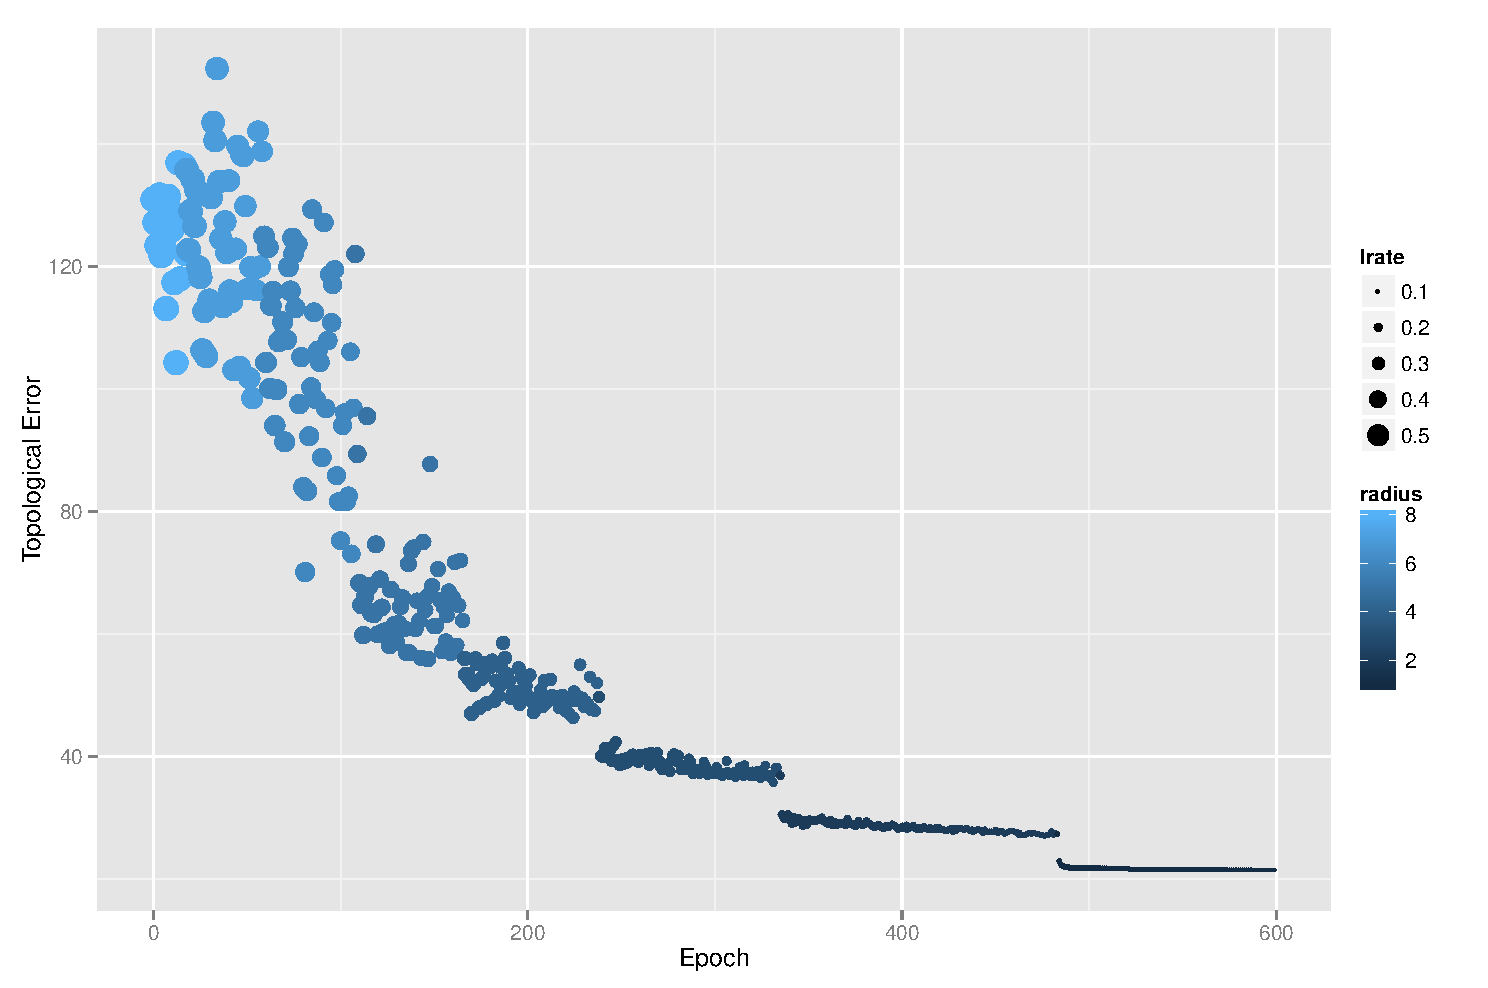
\includegraphics[scale=0.6]{./plots/som/topological_error.pdf}
  \caption{Changes in topological error throughout the SOM training, lrate stands for learning rate, and radius for radius applied to the winning neuron}
  \label{fig:top_error}
\end{figure}

On Figure~\ref{fig:top_error} we can see the evolution of the topological error and how it is converging throwout the training process, as the radius and learning rate are decreasing, and as well as the number of epochs is rising. 

\begin{figure}[h!]
  \centerline{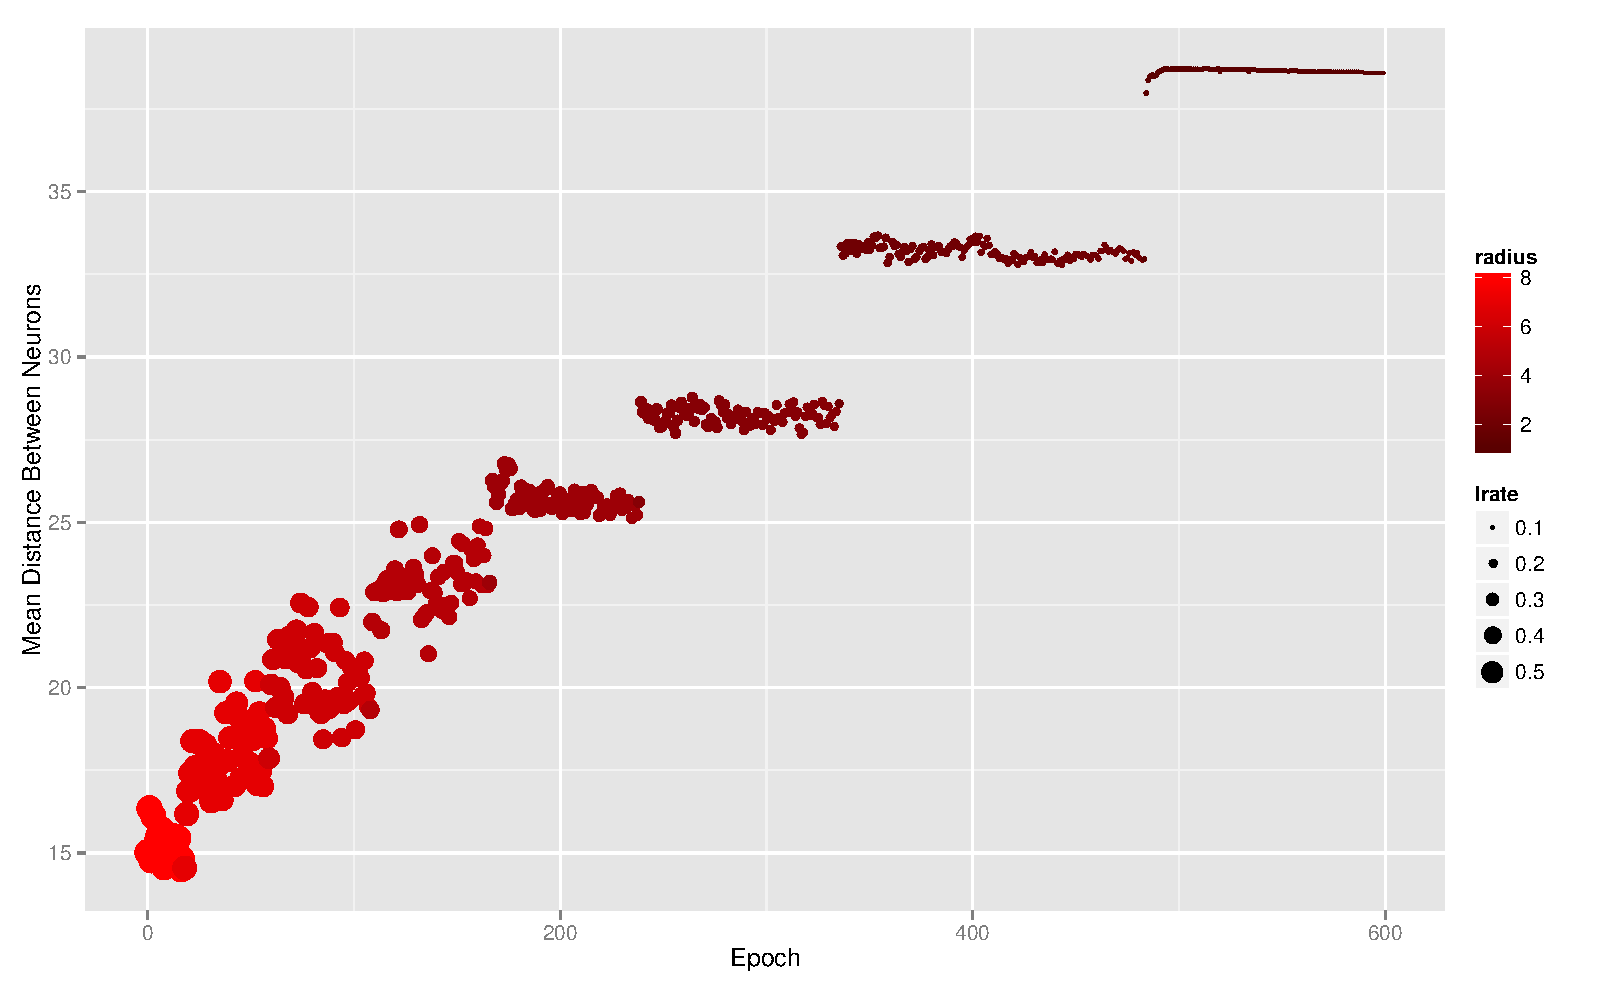
\includegraphics[scale=0.6]{./plots/som/average_distance.pdf}}
  \caption{Changes in the average distance between neurons, throughout the SOM training}
  \label{avg_dist}
\end{figure}

On Figure~\ref{avg_dist} we can see the average distance between neurons increasing. At first this might not look like a desired property, but in fact it is. When the distance between the neurons is increasing and the topological error is decreasing, it means that the neurons are scattering in the output space in order to better identify the input patterns they are responsible for.

During the training of this \ac{SOM}, we analyzed the output space, \ac{U-Matrix} and \ac{Q-Matrix} during the begging, half of the train, and finally at the end of the training.
When comparing the output space on Figure~\ref{chp3:onesom} at the starting of the training, it is possible to see a lot less colors that on Figure~\ref{chp3:threesom}, this is due to the fact that neurons are getting more specified through the training. 
The \ac{U-Matrix} evolves in a way where clusters are almost unnoticeable, which is because each neuron is a cluster by itself, and the distance between it and his neighbors was homogenized throughout the output space. 
The \ac{Q-Matrix} evolves, by becoming whiter which represents that the mean topographic error is becoming smaller. This was already seen before in Figure~\ref{fig:top_error}, but now we can also see which neurons are worst at representing the input patterns.  

\begin{figure}[h!]
  \centering
  \subfigure[Output Space]{
\includegraphics[scale=1]{./images/som_training/1_som.pdf}\label{chp3:onesom}}
  \hspace*{0.5cm}
  \subfigure[U-Matrix]{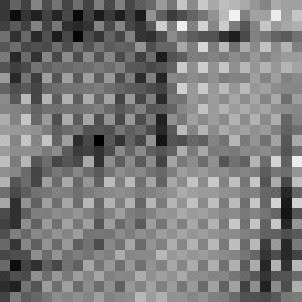
\includegraphics[scale=0.5]{./images/som_training/1_umatrix.pdf}\label{chp3:onematrix}}
  \hspace*{0.5cm}
  \subfigure[Q-Matrix]{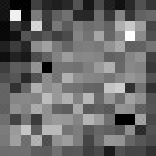
\includegraphics[scale=1]{./images/som_training/1_quantmatrix.pdf}\label{chp3:onetopmat}}
  \hspace*{0.5cm}
  \caption{ SOM state after first epoch of training. Its learning rate is at 0.598, and radius at 8.  }
  \label{fig:}
\end{figure}

\begin{figure}[h!]
  \centering
  \subfigure[Output Space]{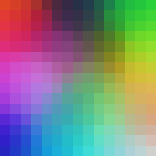
\includegraphics[scale=1]{./images/som_training/2_som.pdf}\label{chp3:onesom}}
  \hspace*{0.5cm}
  \subfigure[U-Matrix]{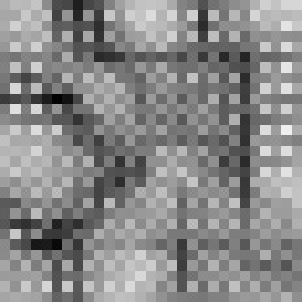
\includegraphics[scale=0.5]{./images/som_training/2_umatrix.pdf}\label{chp3:onematrix}}
  \hspace*{0.5cm}
  \subfigure[Q-Matrix]{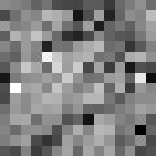
\includegraphics[scale=1]{./images/som_training/2_quantmatrix.pdf}\label{chp3:onetopmat}}
  \hspace*{0.5cm}
  \caption{ SOM state after second epoch of training. Its learning rate is at 0.22, and radius at 3.  }
  \label{fig:}
\end{figure}

\begin{figure}[h!]
  \centering
  \subfigure[Output Space]{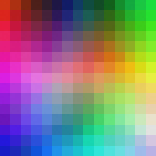
\includegraphics[scale=1]{./images/som_training/3_som.pdf}\label{chp3:threesom}}
  \hspace*{0.5cm}
  \subfigure[U-Matrix]{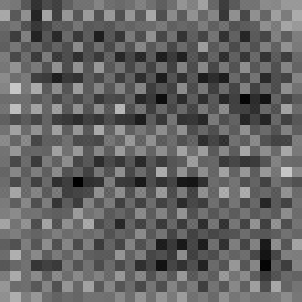
\includegraphics[scale=0.5]{./images/som_training/3_umatrix.pdf}\label{chp3:threematrix}}
  \hspace*{0.5cm}
  \subfigure[Q-Matrix]{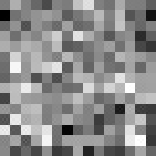
\includegraphics[scale=1]{./images/som_training/3_quantmatrix.pdf}\label{chp3:threetopmat}}
  \hspace*{0.5cm}
  \caption{ SOM state after third epoch of training. Its learning rate is at 0.081, and radius at 1.  }
  \label{fig:}
\end{figure}

In order to see how well the neurons are representing the input patterns, we looked at the \ac{Q-Matrix} and selected the darkest area in order to know which neuron is the worst at representing its input patterns. Afterwards, we printed the input patterns associated to that neuron. This process was graphically represented in Figure~\ref{fig:somtrained} where the colors which represent the input patterns are in fact RGB vector coordinates used during training. It is possible to see that even though this neuron ought to be the worst at representing it input data, he represents it quite well as they are all shades of red. 
It is important to know that all of this visualization can only be made due to the fact that, we are working with arrays with three dimension and values comprised between 0 and 255 --- which makes it possible for them to be presented as RGB images. 

\begin{figure}[h!]
  \centering
  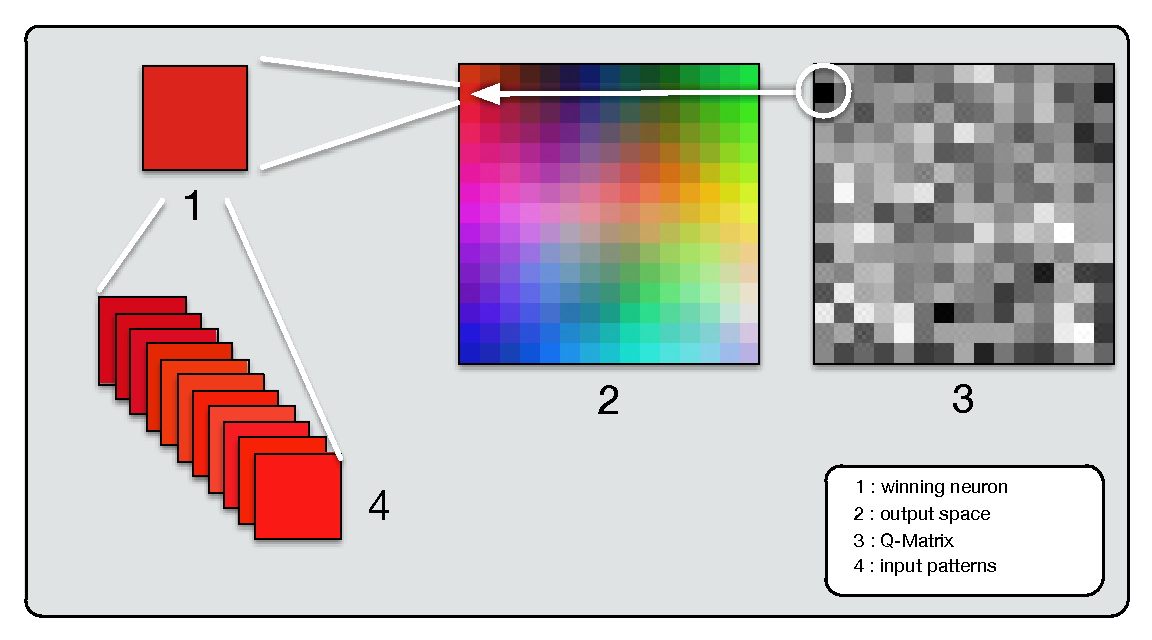
\includegraphics[width=0.8\linewidth]{./images/som_trainned.pdf}
  \caption{Input patterns associated with the neuron with maximum topological error --31. Even though the neuron has the biggest topological error of all neurons, it still has a good representation of the input patterns. The colors in this image are not figurative, and represent the entities at the end of training.  }
  \label{fig:somtrained}
\end{figure}

\subsection{Benchmarking}
\label{sub:benchmarking}
The \ac{SOM} was not created with the purpose of being extremely fast, for that there are already very good implementations like \citet{somoclu} distributed library for \ac{SOM} or \citet{rsom} R kohonen package which implements the training algorithm in C, and only exposes the interface in the high level language R.  
Being purely written in a higher level language, the \ac{SOM} framework enables researchers and programmers to write training algorithms very fast. For example, the code necessary for training the colored vectors on the previous subsection can be seen in Figure~\ref{fig:rubysom}.

\begin{figure}[h!]
  \centering
  \begin{boxedverbatim}
  ## Create a new SOM object
  som = SOM::SOM.new output_space_size: 15, epochs: 1500

  ## Generate 1500 random input patterns
  som.input_patterns = 1500.times.inject([]){ |arr| arr << Array.new(3){ rand(0..255) }; arr  }

  ## Start training
  som.exec!
  \end{boxedverbatim}
  \caption{ Ruby code necessary for training a SOM with 1500 input patterns.  }
  \label{fig:rubysom}
\end{figure}

In order to better understand the amount of data \ac{SOM} framework is able to handle, we benchmarked it on the same machine used in Table~\ref{tab:mac_test}. The framework was tested against multiple sizes of output space and input patterns, multiple numbers of input patterns, and multiple numbers of epochs. 
The results were summarized on Figure~\ref{fig:benchmarkingsom}, where it is possible to see on the upper quadrant that if all parameters increase, \ac{SOM} training will suffer as well.

\begin{figure}[h!]
  \centering
  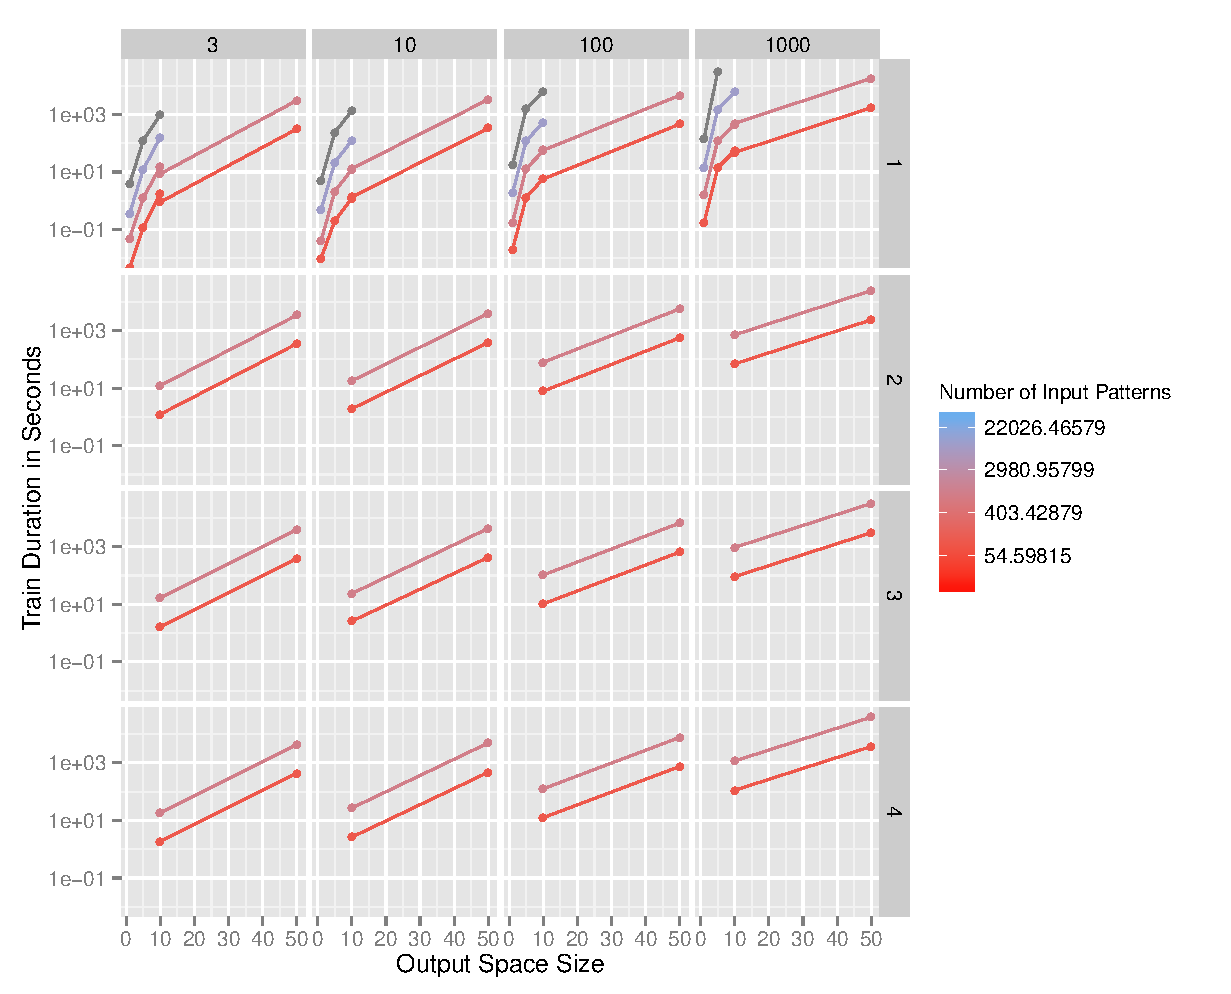
\includegraphics[width=0.8\linewidth]{./plots/som/benchmarking.pdf}
  \caption{SOM framework train duration, influenced by output space size in the XX axis, duration of the training on the YY axis, number of epochs in the right, size of input patterns on top, and number of input patterns on the right in color from red to blue.}
  \label{fig:benchmarkingsom}
\end{figure}


\section{Homophilic SOM}
\label{sec:homophilic_som}

In order bring the concept of homophily --- which have proved to be present on social networks~\cite[]{Wehrens2007}  --- to clustering socially connected data, on Section \ref{sec:algorithm_changes} we suggested some alterations to the default \ac{SOM} algorithm. These modifications were mainly applied to the output space, where each neuron started to represent a user, and his neighborhood is comprised of his social relations.

These features were implemented into the \ac{SOM} framework described in the previous chapter. The data used to train the homophilic \ac{SOM} can be seen in Table \ref{tab:homosom}. The training was performed on a machine with the characteristics show in Table \ref{tab:acer_test}.

\begin{table}[H]
  \caption{Second test machine specs}
  \label{tab:acer_test}
  \begin{center}
    \begin{tabular}{|c|c|}
      \hline
      Operative System & Ubuntu 13.10\\
      \hline
      Memory           & 16GB DDR3 Synchronous 1600 MHz      \\
      \hline
      Processor        & Intel(R) Core(TM) i7-3770 CPU @ 3.40GHz \\
      \hline
      Hard Drive       & 2TB HDD  \\
      \hline
    \end{tabular}
  \end{center}
\end{table}

\begin{table}[H]
  \caption{Homophilic SOM characteristics}
  \label{tab:homosom}
  \begin{center}
    \begin{tabular}{|c|c|}
      \hline
      Number of tweets & 1575 \\
      \hline
      Number of users & 25  \\
      \hline
      Output space size        & 100 \\
      \hline
      Input space size       & 3342 words  \\
      \hline
      Words used for clustering & Hashtags, comon and proper nouns  \\
      \hline
      SVM reductors used & all  \\
      \hline
      Training duration & 74h \\
      \hline
      Initial number of hops & 4 \\
      \hline
    \end{tabular}
  \end{center}
\end{table}


It is not possible to draw a \ac{U-Matrix} due to the fact that the output space is no longer a rectangular matrix, but a graph. Also drawing, the \ac{Q-Matrix} is possible, but the disposition of the neurons will not represent the actual disposition in the graph. This can still be useful to easily visualize which neurons are better at representing their input patterns. 

Looking at the results, there are a lot of different topics of clusters. There were neurons clearly responsible to identify music, like it can be seen on Figure~\ref{clust:tech}. On Figure~\ref{clust:music} we can see a cluster about tech and programing, the most surprising part about this cluster is that the tweet about the banana phone, is actually inserted into the tech topic --- it was tech project presented at codebits. 
On the other hand, some clusters of people saying that they have posted photos on facebook, or that they've liked youtube videos were also found. Even though they can be considered topics, their relevance is not very high.

\begin{figure}[h!]
  \centering
  \subfigure[Cluster about tech and programing]{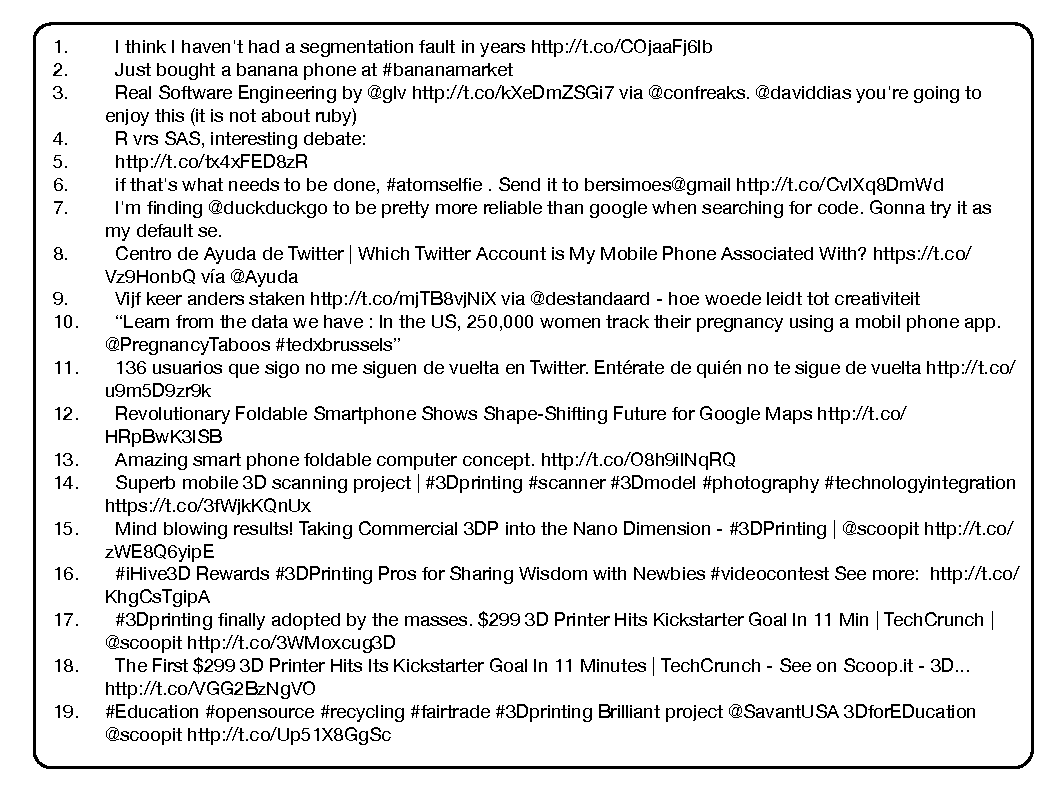
\includegraphics[scale=0.6]{./images/1clustertech.pdf}\label{clust:tech}}
  \hspace*{0.5cm}
  \centering
  \subfigure[Cluster about music]{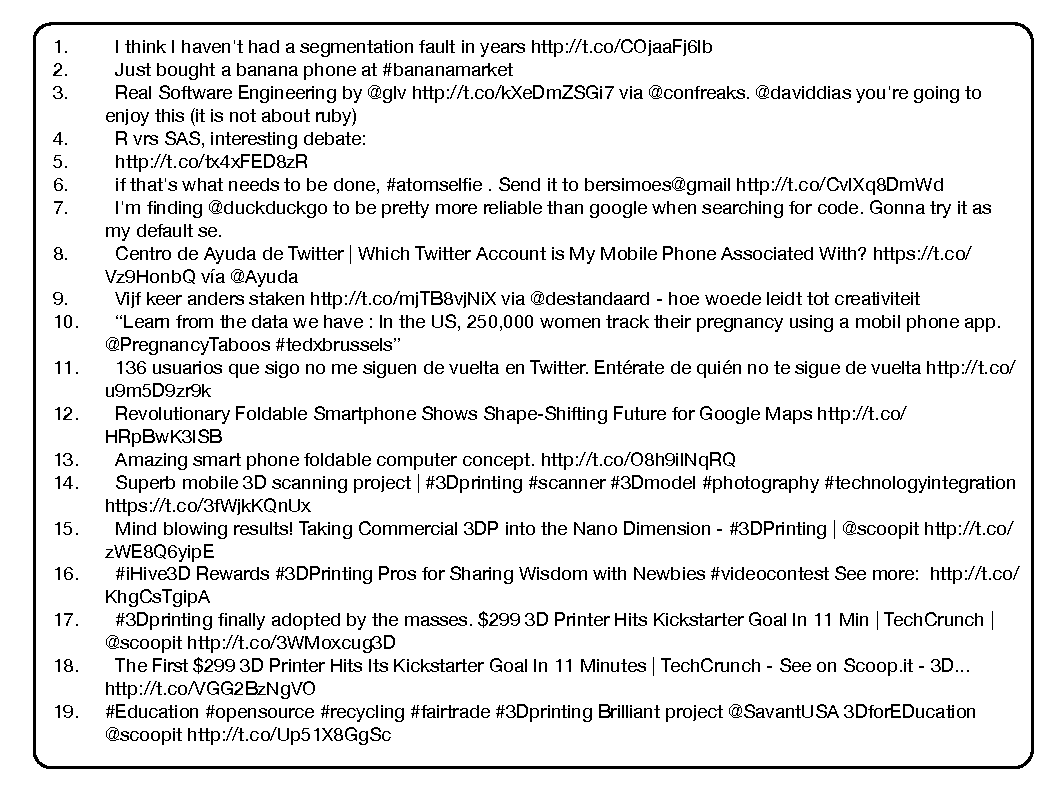
\includegraphics[scale=0.6]{./images/2clustertech.pdf}\label{clust:music}}
  \label{fig:clusters}
  \caption{Two clusters with different topics}
\end{figure}

\section{Conclusions}

% Ensure that the next chapter starts in a odd page
\cleardoublepage
 %\subsection{Twitter Dataset}
%\label{subsec:twitter_dataset}

%As can be seen in Figure~\ref{fig:json_tweet_user} no information about the social relations of the user which emitted the tweet are present. Therefor in order to retrieve the social network in which a user is contained, it will be necessary to connect to the Twitter API. Crawling twitter is discussed in further depth in Chapter~\ref{chap:crawling_twitter}.  


%In order to better understand the dataset at hand, all the \ac{JSON} files where converted into \ac{CSV}in a way to reduce the size of the dataset. While tweets where being converted, \ac{URL} where removed --- since most of them where minified in order to fit in less that 140 characters, without translating the minified URL, not a lot of information can be gathered. Also, all tweets that where not identified as being in English where also removed. The tweet shown in \ac{JSON} format in Figure~\ref{fig:json_tweet} is converted to \ac{CSV} in Figure~\ref{fig:csv_tweet}.
 
%%%%%% REMOVED STUFF
%\subsection{Topology Preservation} 
%\label{sub:topology_preservation}
%The Self-Organizing Map performs a mapping from the n-dimensional input space into the two dimensional output space and where resides one the most fascinating characteristics, which is that the output map tries to preserve the topology from the input space. This grants the SOM algorithm a way to visualize high-dimensional data that other neural networks or clustering algorithms don't have. Even though this is true, sometimes during training it is not possible to preserve the topology of the network.
%Thus topology preservation can be measured through the Topographic error~\citet{Kiviluoto1996} which is the proportion of all data vectors for which first and second BMUs \footnote{unit that is closest to the winning neuron. BMU Best fitting unit } are not adjacent units.
%In this project the Topographic Error will be calculated for all SOM implementations and VSM usages in order to understand if the representation of the SOM output space is well defined.

 %\begin{itemize}
  %\item show UMatrixes and multiple steps map trainning of the SOM library trainnig
  %\item show metrics for the crawller, tweets per second, users persecond, size of the dump a long the time.
  %\item compare my som library with other som libraries: training velocity with diferent parameters, map after trainned.
  %\item Compare Homophilic-SOM results with non homophilic: UMatrixes, cluster results, Quantization error, jacknife. 
%\end{itemize}
%%\section{Evaluation Metrics} 
%%\label{sec:evaluation_metrics}
%Evaluation of the topic detection on Tweets will be made in two distinct ways. The first way will focus on  binary classification using the precision and recall metrics, and will be described in Subsection~\ref{sub:testing_for_precision_and_recall}. The second way will focus on statistically testing the SOM learning process and the computed trained network. This testing process will be described in Subsection~\ref{sub:cluster_quality_testing}. 

%\section{Testing for Precision and Recall} 
%\label{sec:testing_for_precision_and_recall}
%Precision and Recall are both ways to measure the rate of right guesses made by the trained SOM network, and are defined in the following way:
%\begin{itemize}
  %\item \textbf{Precision:} Fraction of retrieved instances that where relevant 
    %\begin{equation}
  precision = \frac{|{relevant\;documents}\cap{retrieved\;documents}|}{{retrieved\;documents}}
\end{equation} 

  %\item \textbf{Recall:} Fraction of relevant instances that where retrieved
    %\begin{equation}
  recall = \frac{|{relevant\;documents}\cap{retrieved\;documents}|}{{relevant\;documents}} 
\end{equation} 

%\end{itemize}
 
%In order to calculate Precision and Recall we need to have the \emph{relevant documents} and the \emph{retrieved documents}. The \emph{relevant documents} are rather hard to determine because they need to be categorized by humans, which is an expensive task.
